% TikZ pictures in boxes that resize them (nested, mirrored, turned over,
% and not uniformly, also in a figure), an \includegraphics and text in
% such a box, a scaled box in a picture, inline pictures with a baseline
% (one in a node of a picture without), and a commutative diagram in
% display math.
\documentclass{article}
\usepackage{tikz}
\usepackage{tikz-cd}
\usepackage{graphicx}
\begin{document}
\section{Scaled}
Half: \scalebox{0.5}{\tikz{\draw (0,0) rectangle (4,2); \node at (2,1) {Half};}}

Full: \tikz{\draw (0,0) rectangle (4,2); \node at (2,1) {Full};}

Text width: \resizebox{\textwidth}{!}{\tikz{\draw (0,0) rectangle (20,2); \node at (10,1) {Wide};}}

\resizebox{!}{1cm}{\tikz{\draw (0,0) rectangle (4,2);}}

Quarter: \scalebox{0.5}{\scalebox{0.5}{\tikz{\draw (0,0) rectangle (4,2); \node at (2,1) {Quarter};}}}

Mirrored: \reflectbox{\tikz{\draw (0,0) rectangle (4,2); \node at (2,1) {Mirrored};}}

Stretched: \scalebox{2}[1]{\tikz{\draw (0,0) rectangle (4,2); \node at (2,1) {Stretched};}}

Photo: \scalebox{0.5}{
\includegraphics[alt={halved}, width=100pt]{test-picture.png}}

Text: \scalebox{2}{Big}
\section{Baseline}
Text \tikz[baseline=(X.base)]{\node[draw] (X) {base};} and
\tikz[baseline=-0.5ex]{\draw (0,0) circle (0.3);} and
\tikz{\draw (0,0) circle (0.3);} after.

Text \tikz[baseline=(Y.base)]{\node (Y) {bare};} and
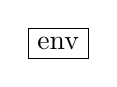
\begin{tikzpicture}[baseline=(Z.base)]\node[draw] (Z) {env};\end{tikzpicture}
and \scalebox{2}{\tikz[baseline=-0.5ex]{\draw (0,0) circle (0.15);}} after.

Text \tikz{\node[draw] {in \tikz[baseline=-0.5ex]{\draw (0,0) circle (0.1);} a node};} after.
\section{Diagram}
\[
\begin{tikzcd}
A \arrow[r, "f"] & B
\end{tikzcd}
\]
\section{More}
\resizebox{\textwidth}{!}{\begin{tikzpicture}\draw (0,0) rectangle (20,2);\end{tikzpicture}}

Turned over: \scalebox{1}[-1]{\tikz{\draw (0,0) rectangle (2,1); \node at (1,0.5) {Up};}} after.

Node: \tikz\node{\scalebox{2}{x}};
\begin{figure}
\centering
\scalebox{2}[1]{\tikz{\draw (0,0) rectangle (4,2); \node at (2,1) {Stretched};}}
\reflectbox{\tikz{\draw (0,0) rectangle (4,2); \node at (2,1) {Mirrored};}}
\end{figure}
\end{document}
